
% \begin{figure*}[!htb]
%     \centering
%     \subfigure[]{
% 	    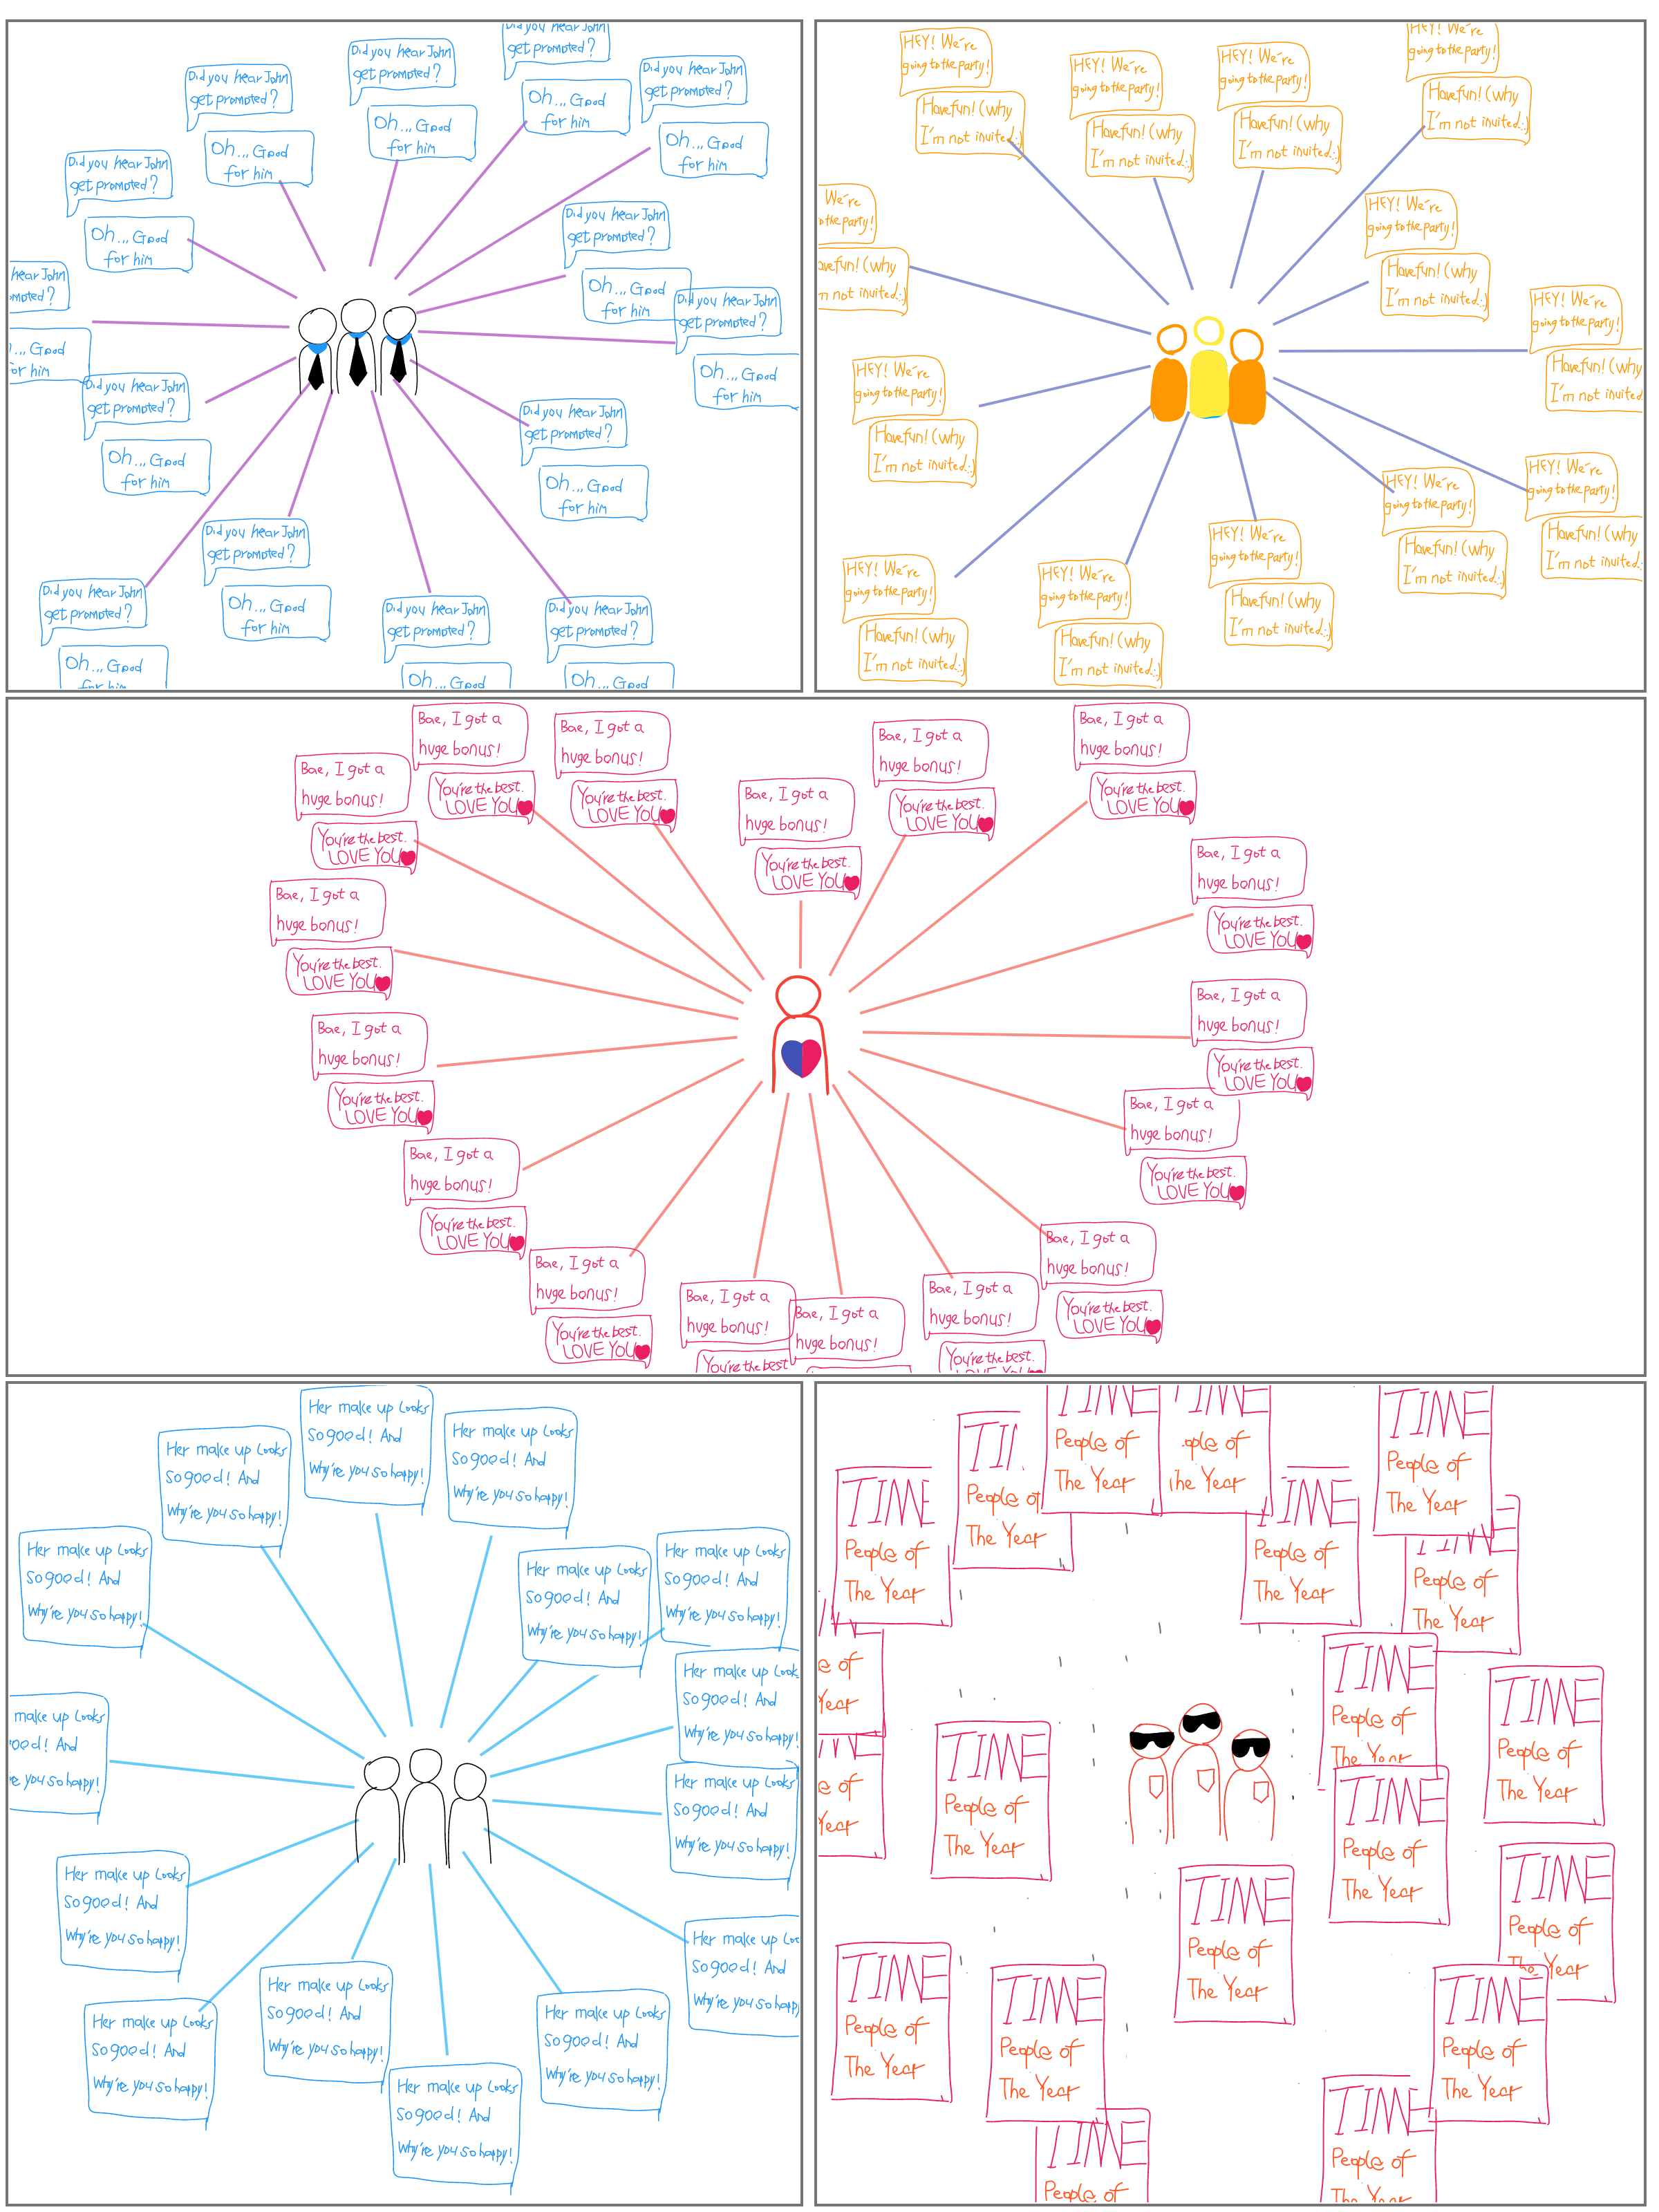
\includegraphics[width=0.25\textwidth]{figures/people}
%     }
%     \hfill{}
%     \subfigure[]{
%     	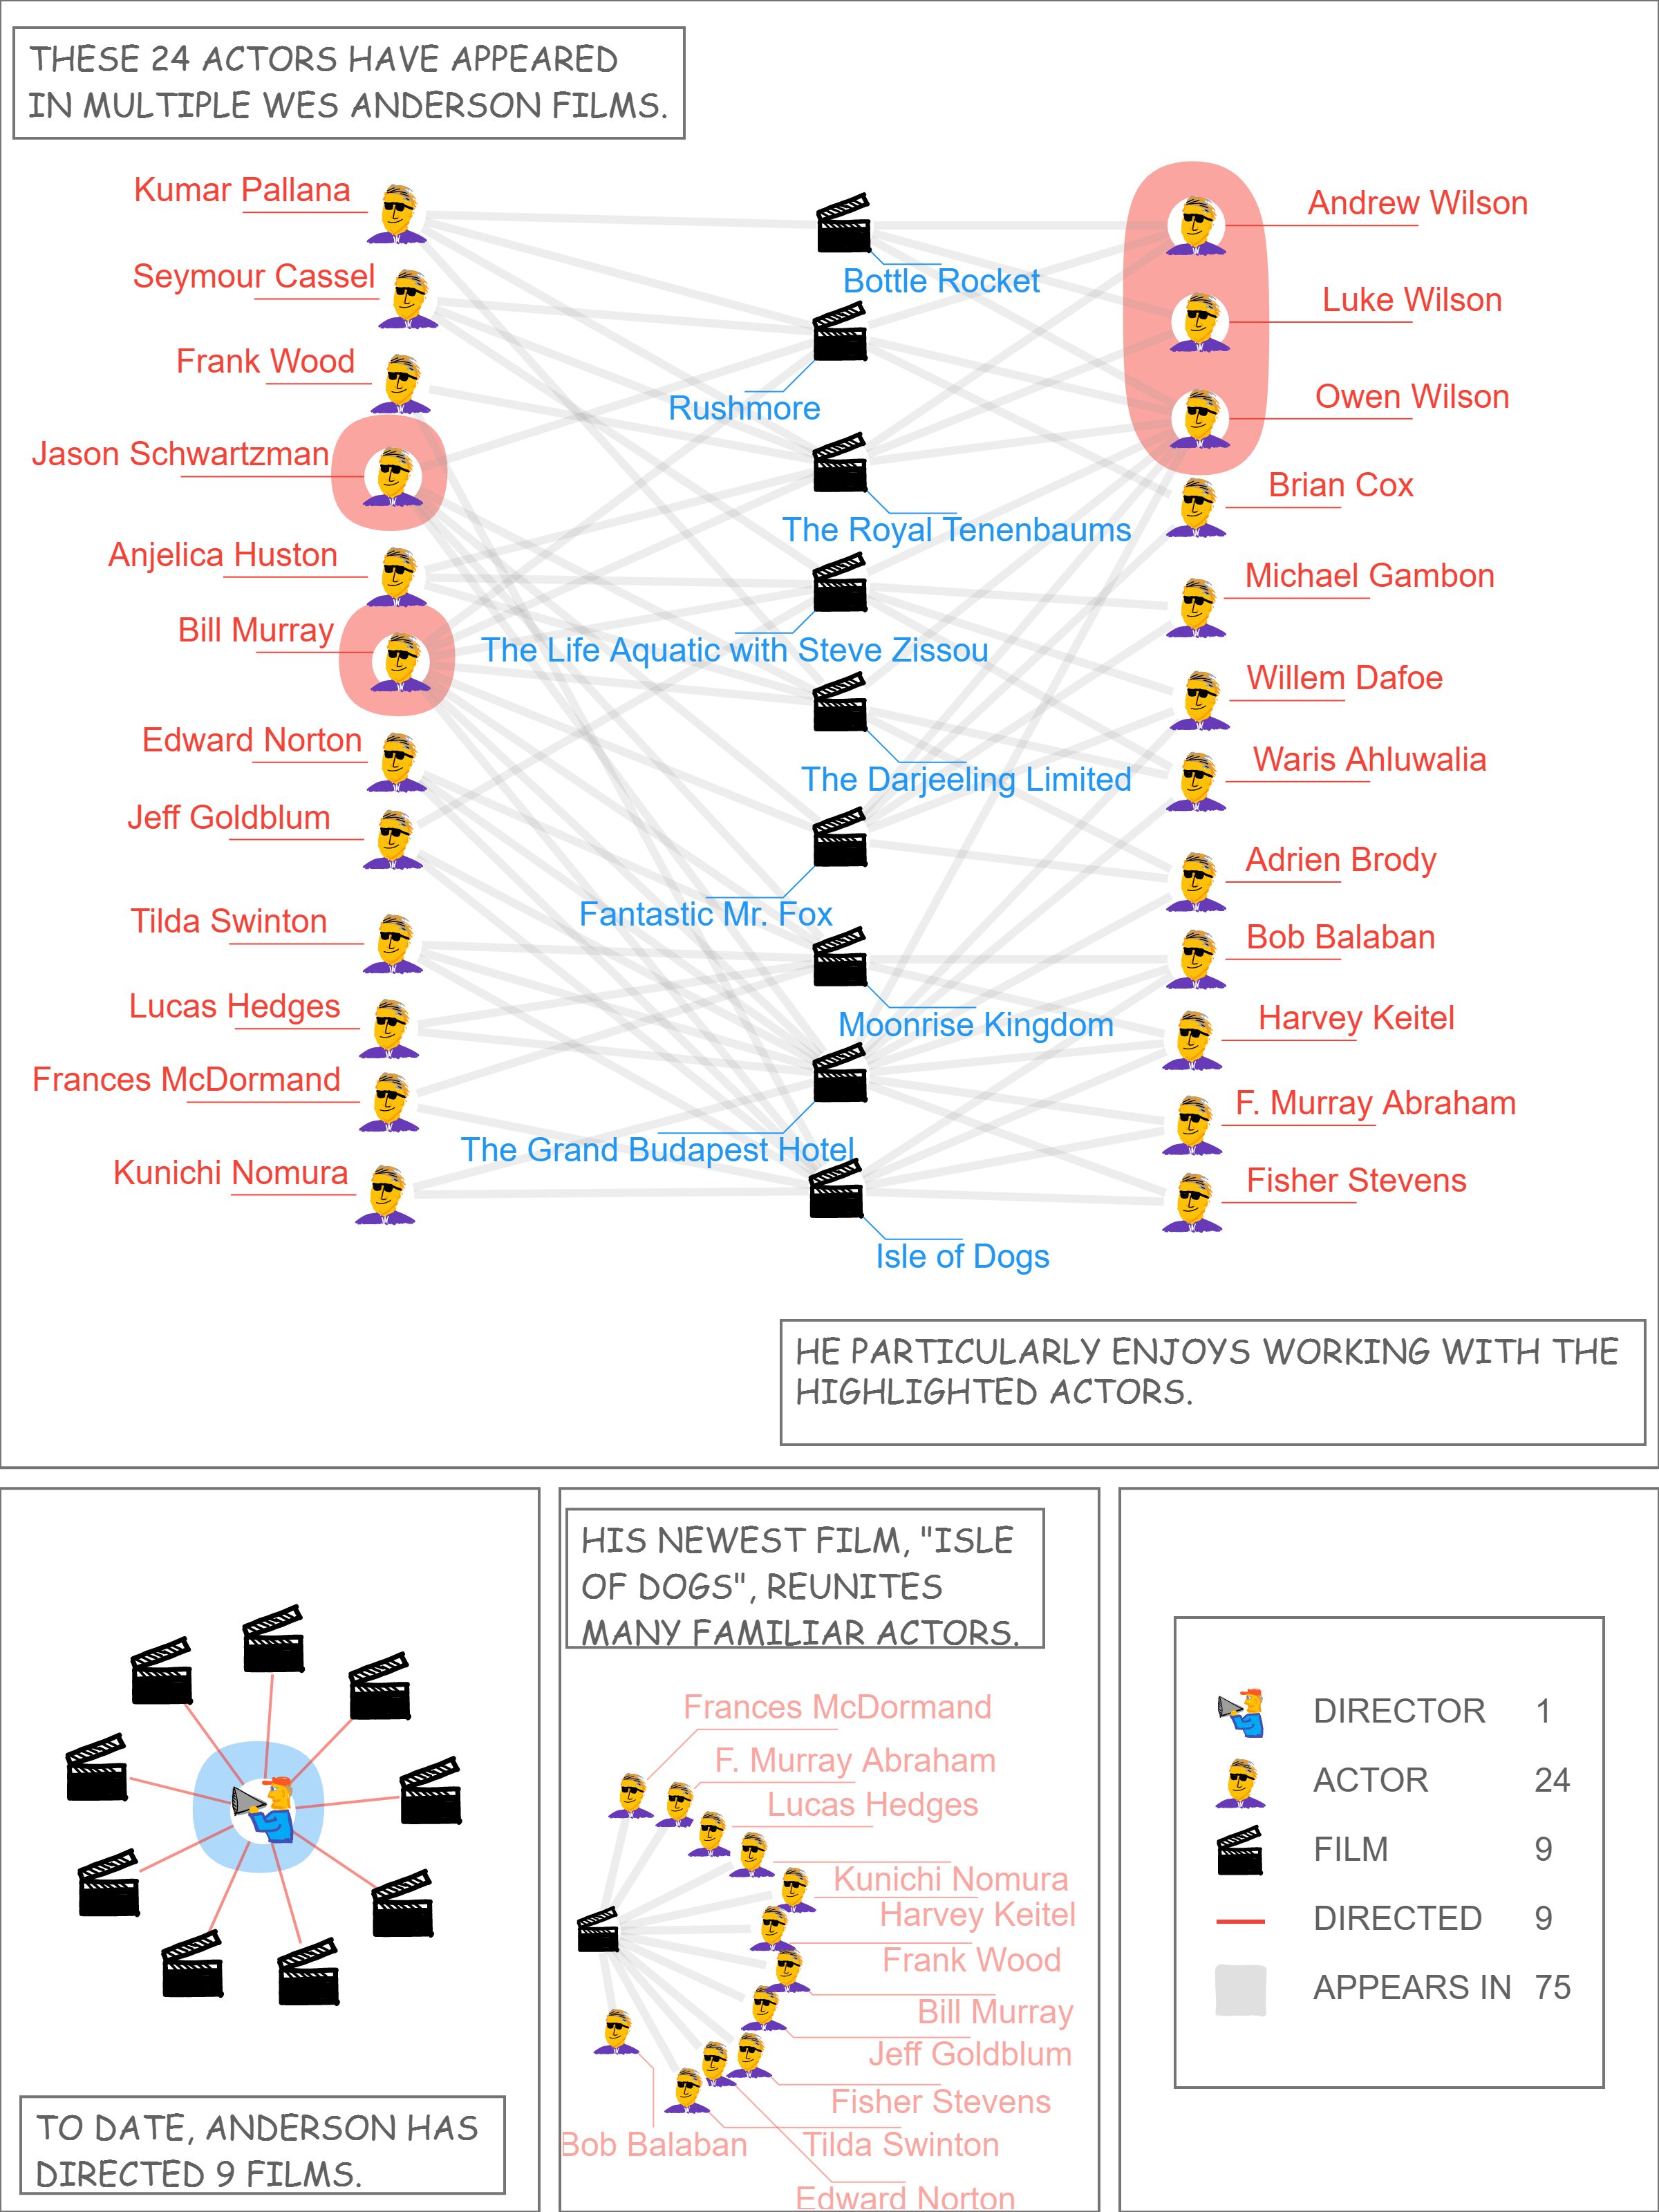
\includegraphics[width=0.25\textwidth]{figures/wes_anderson} 
%     }
%     \hfill{}
%     \subfigure[]{
% 	    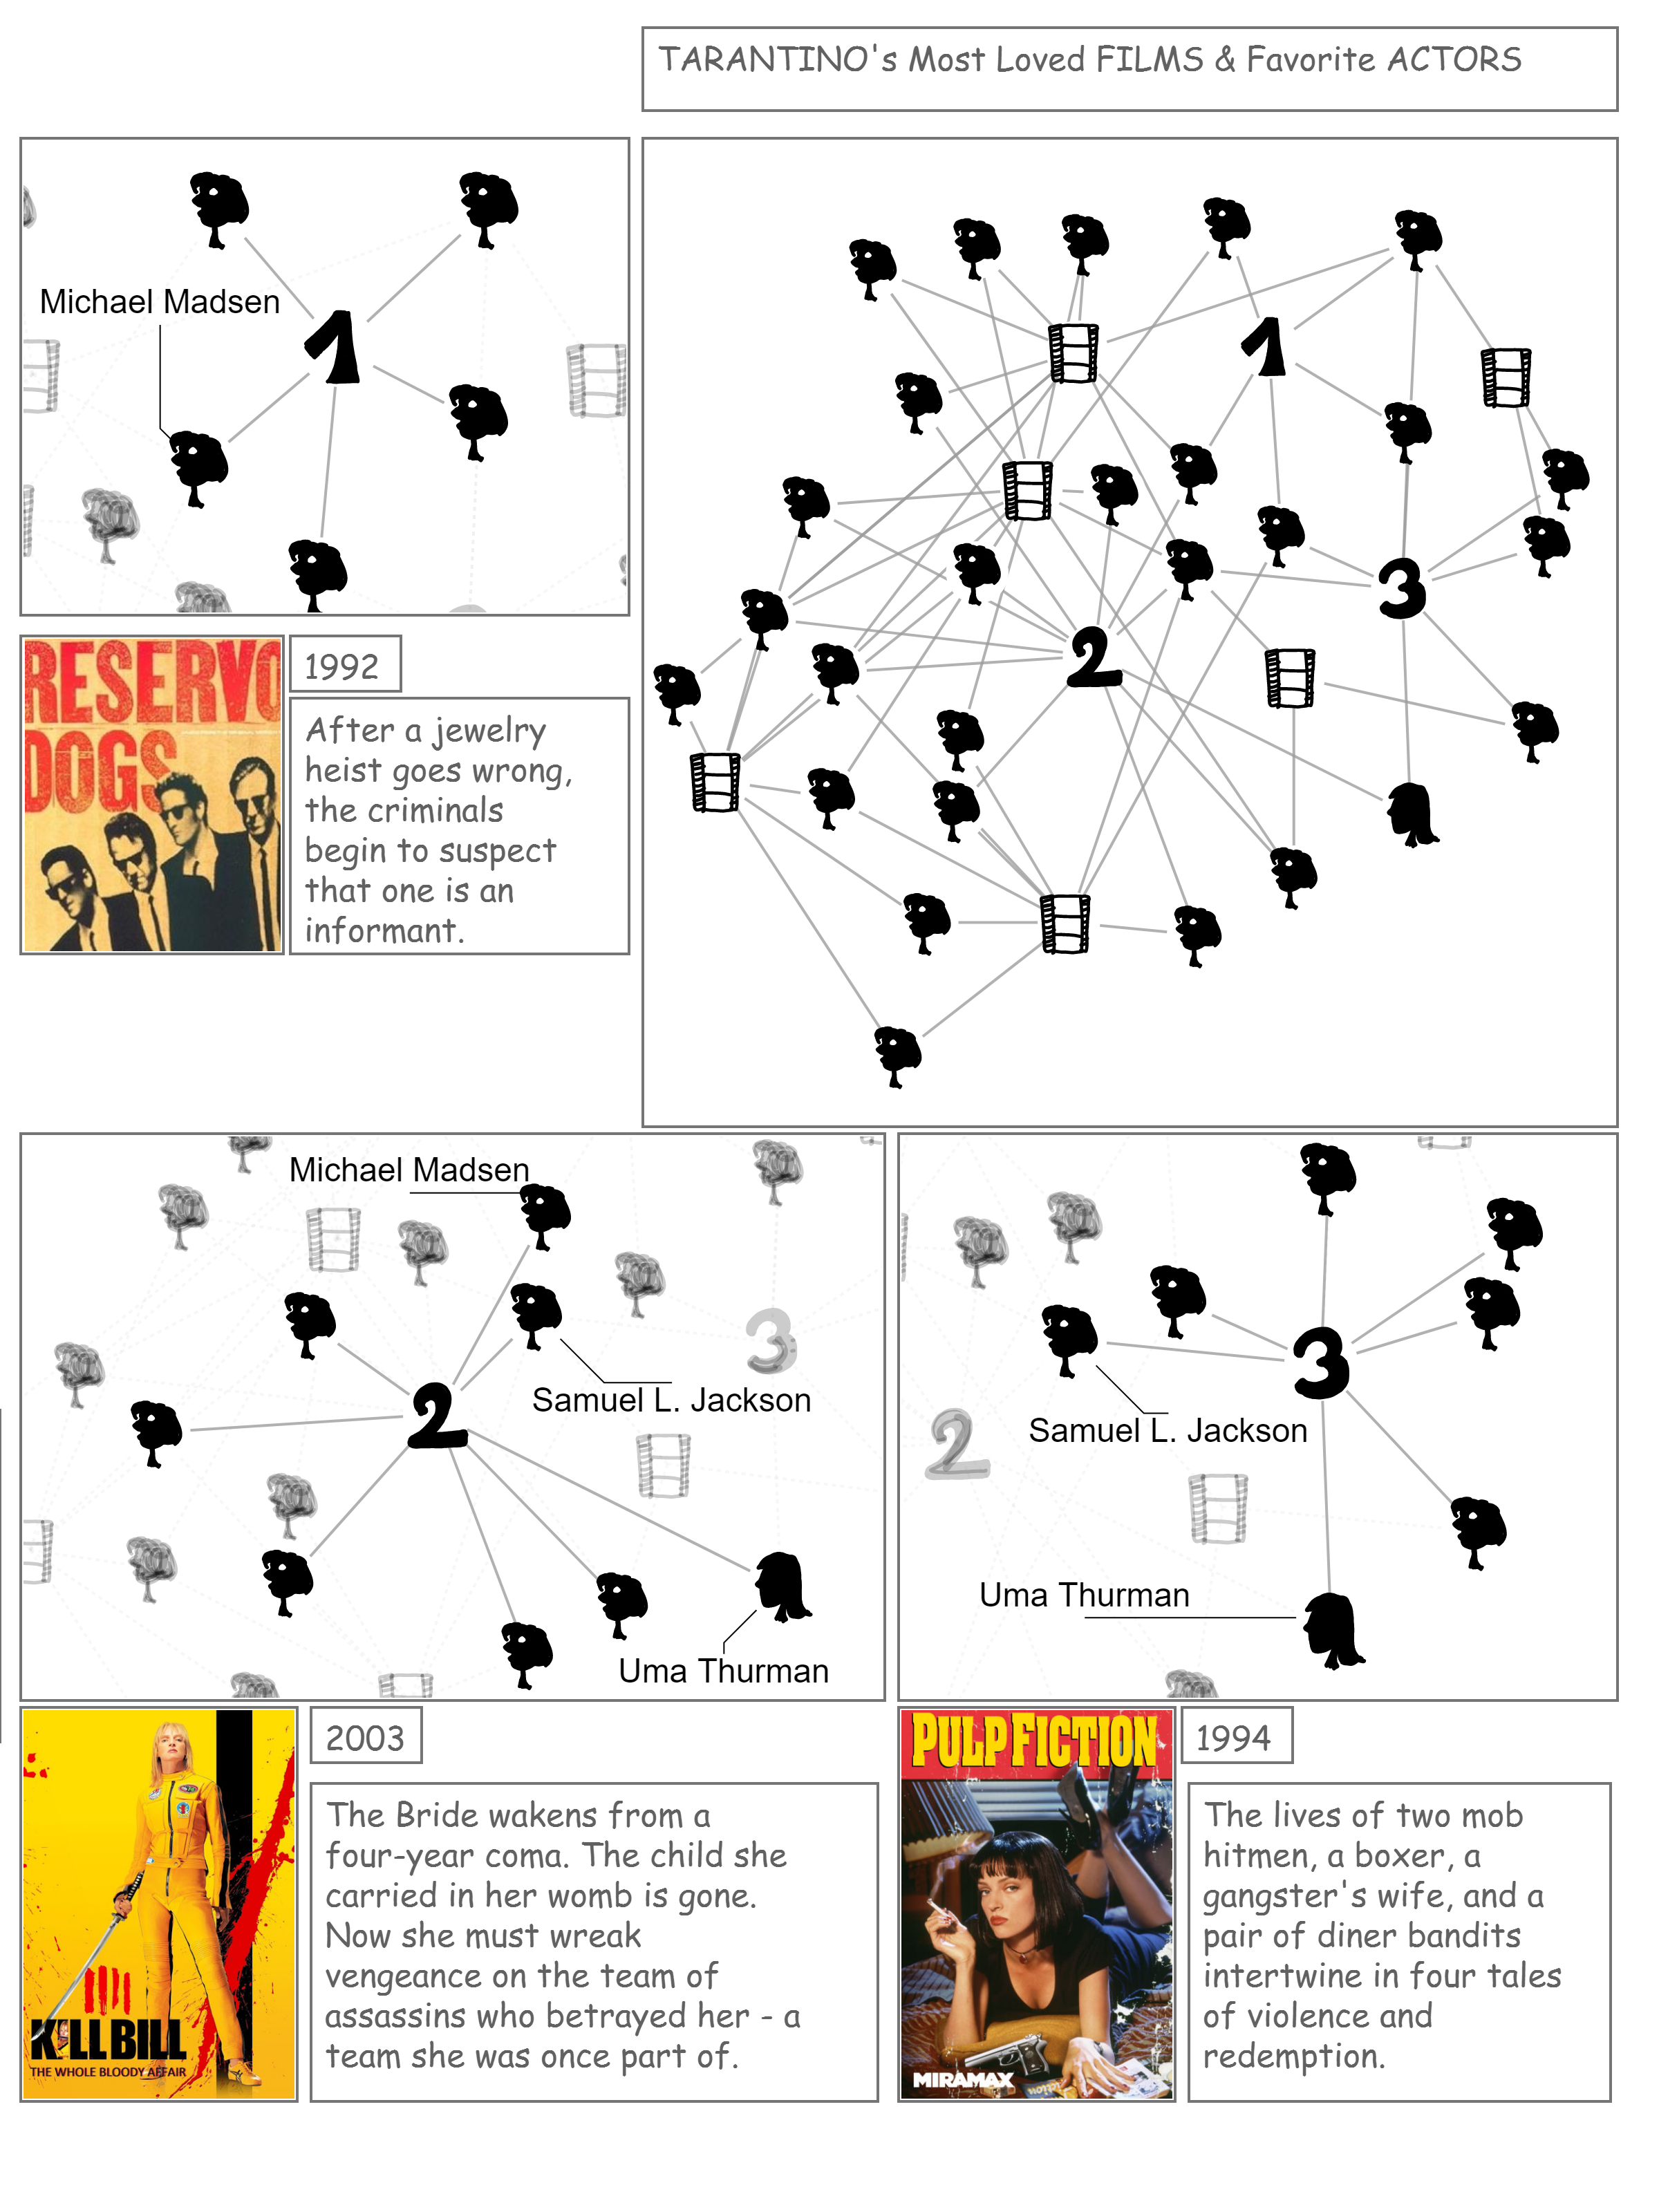
\includegraphics[width=0.25\textwidth]{figures/tarantino}
% 	}
%     \hfill{}
%     \subfigure[]{
% 		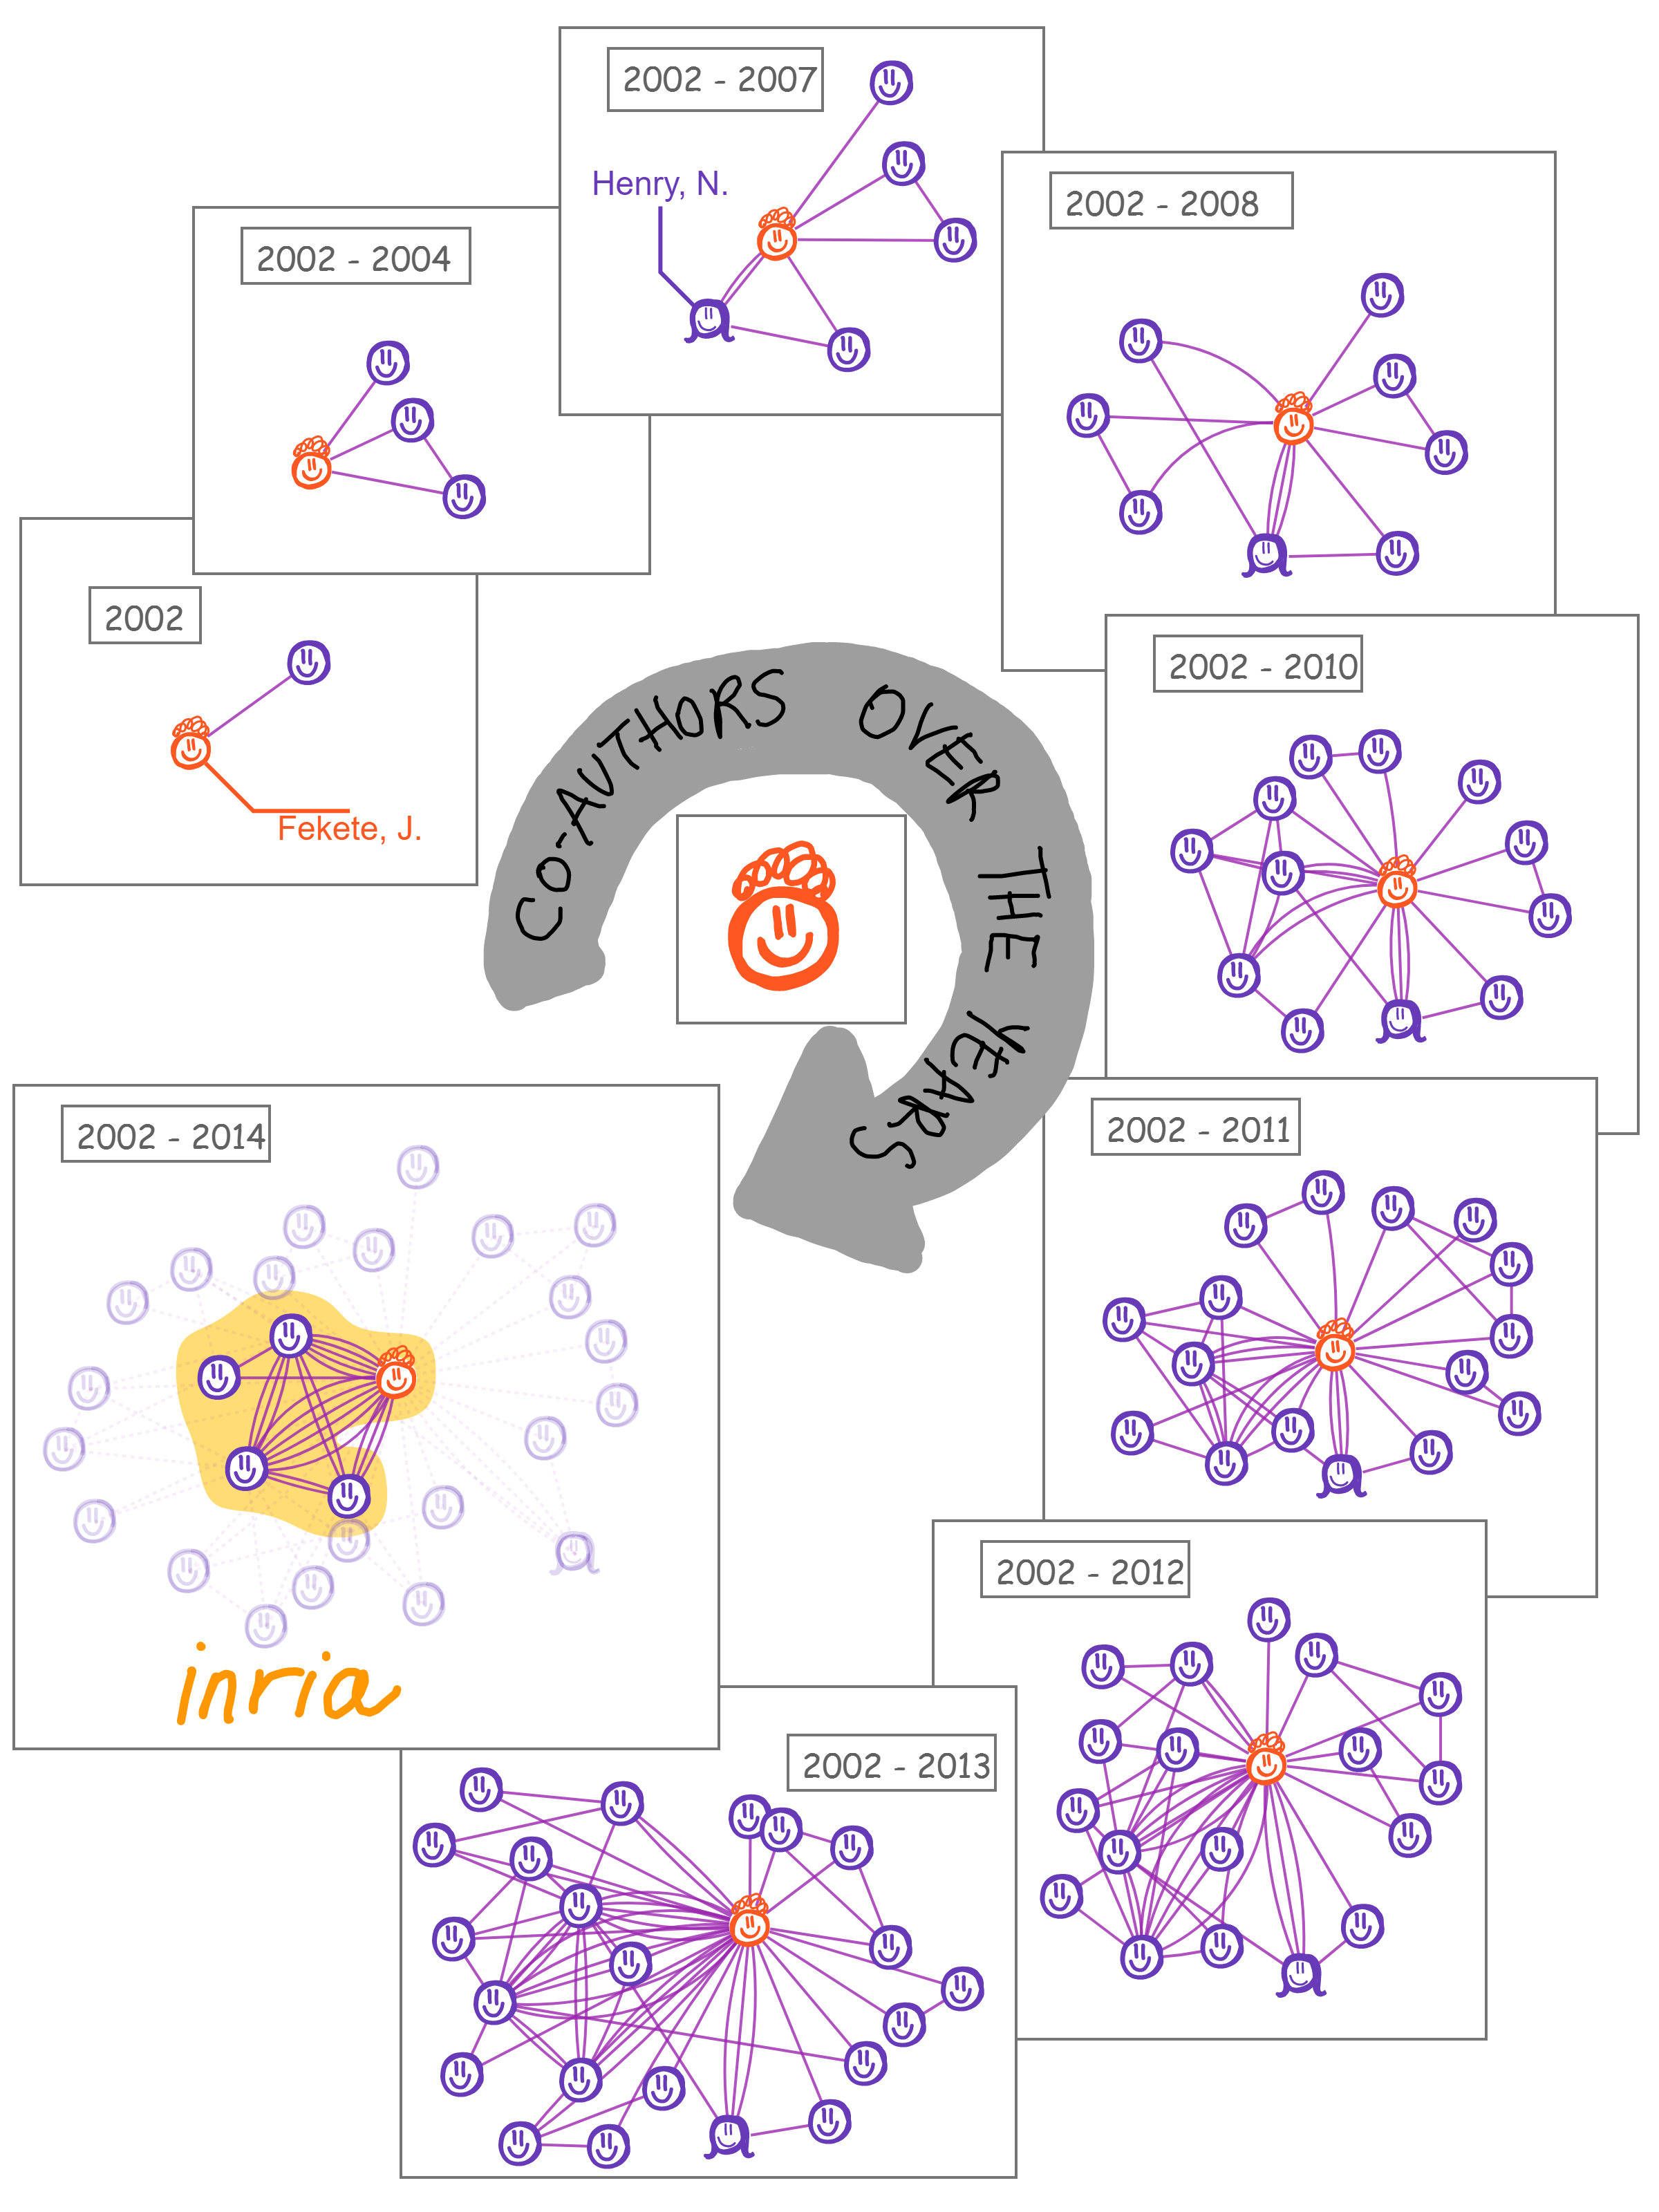
\includegraphics[width=0.25\textwidth]{figures/fekete}
%     }
%     \subfigure[]{
% 		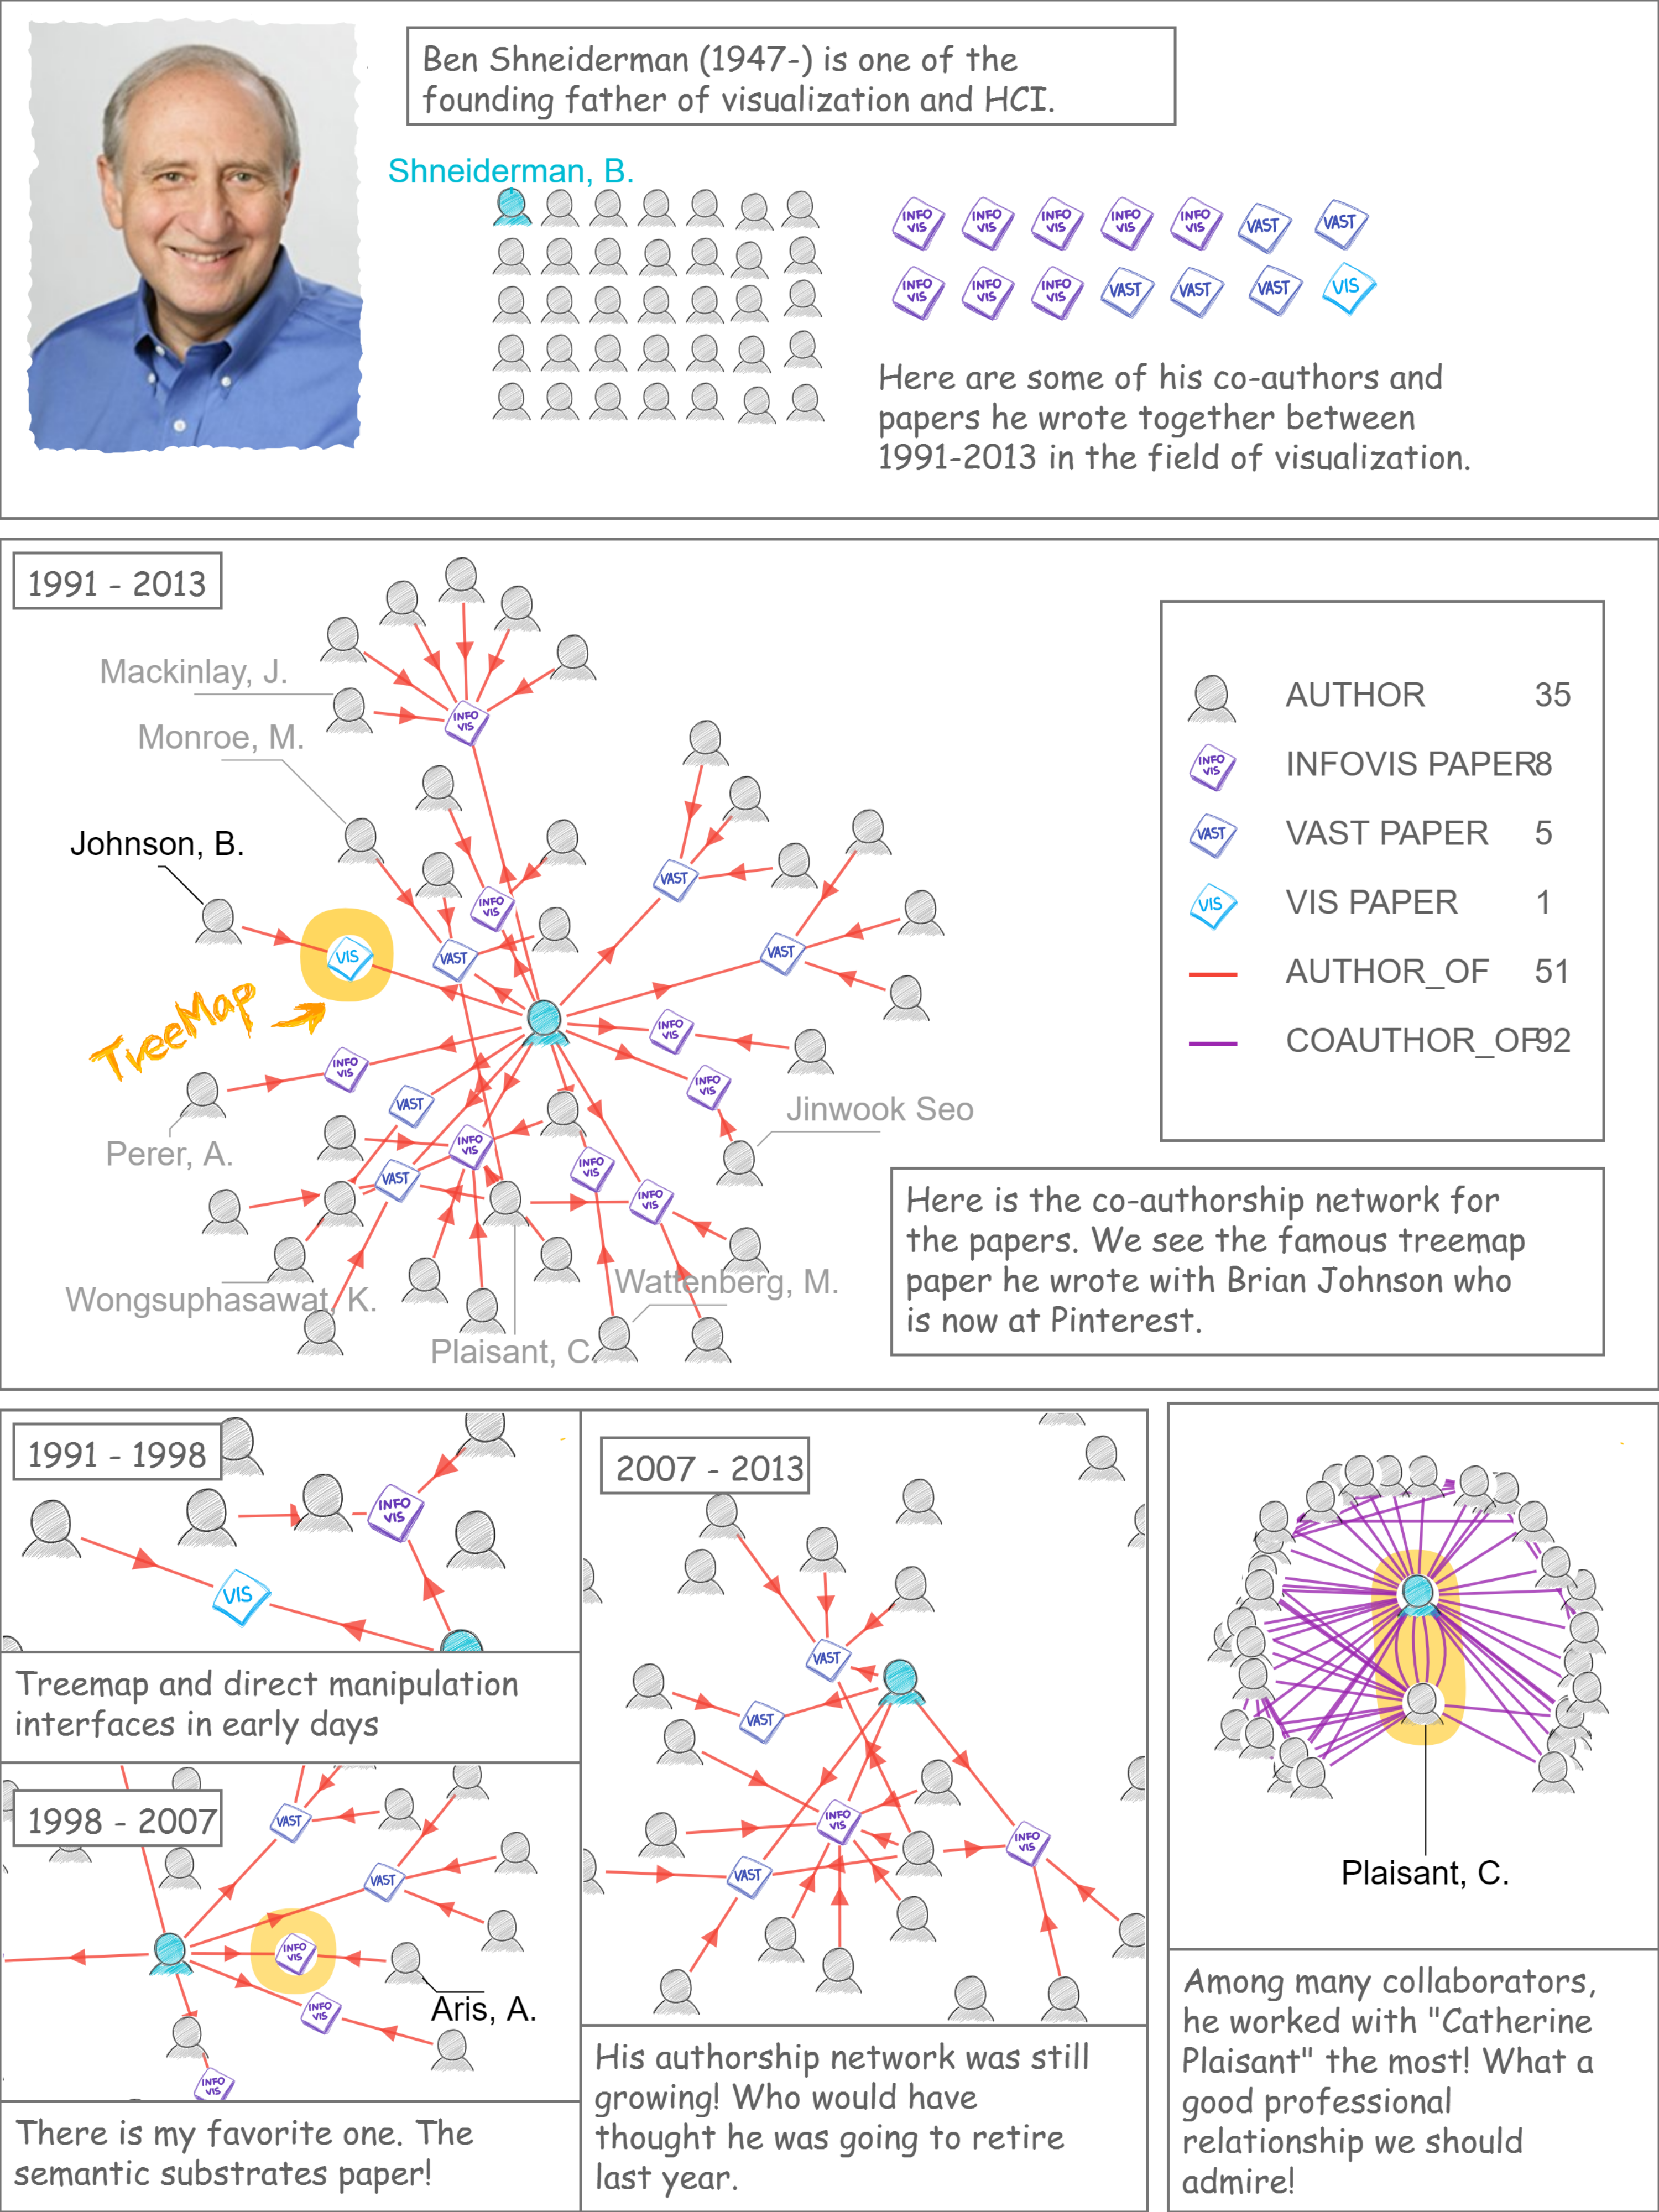
\includegraphics[width=0.25\textwidth]{figures/ben-comics}     
%     }
%     \hfill{}
%     \subfigure[]{
%   		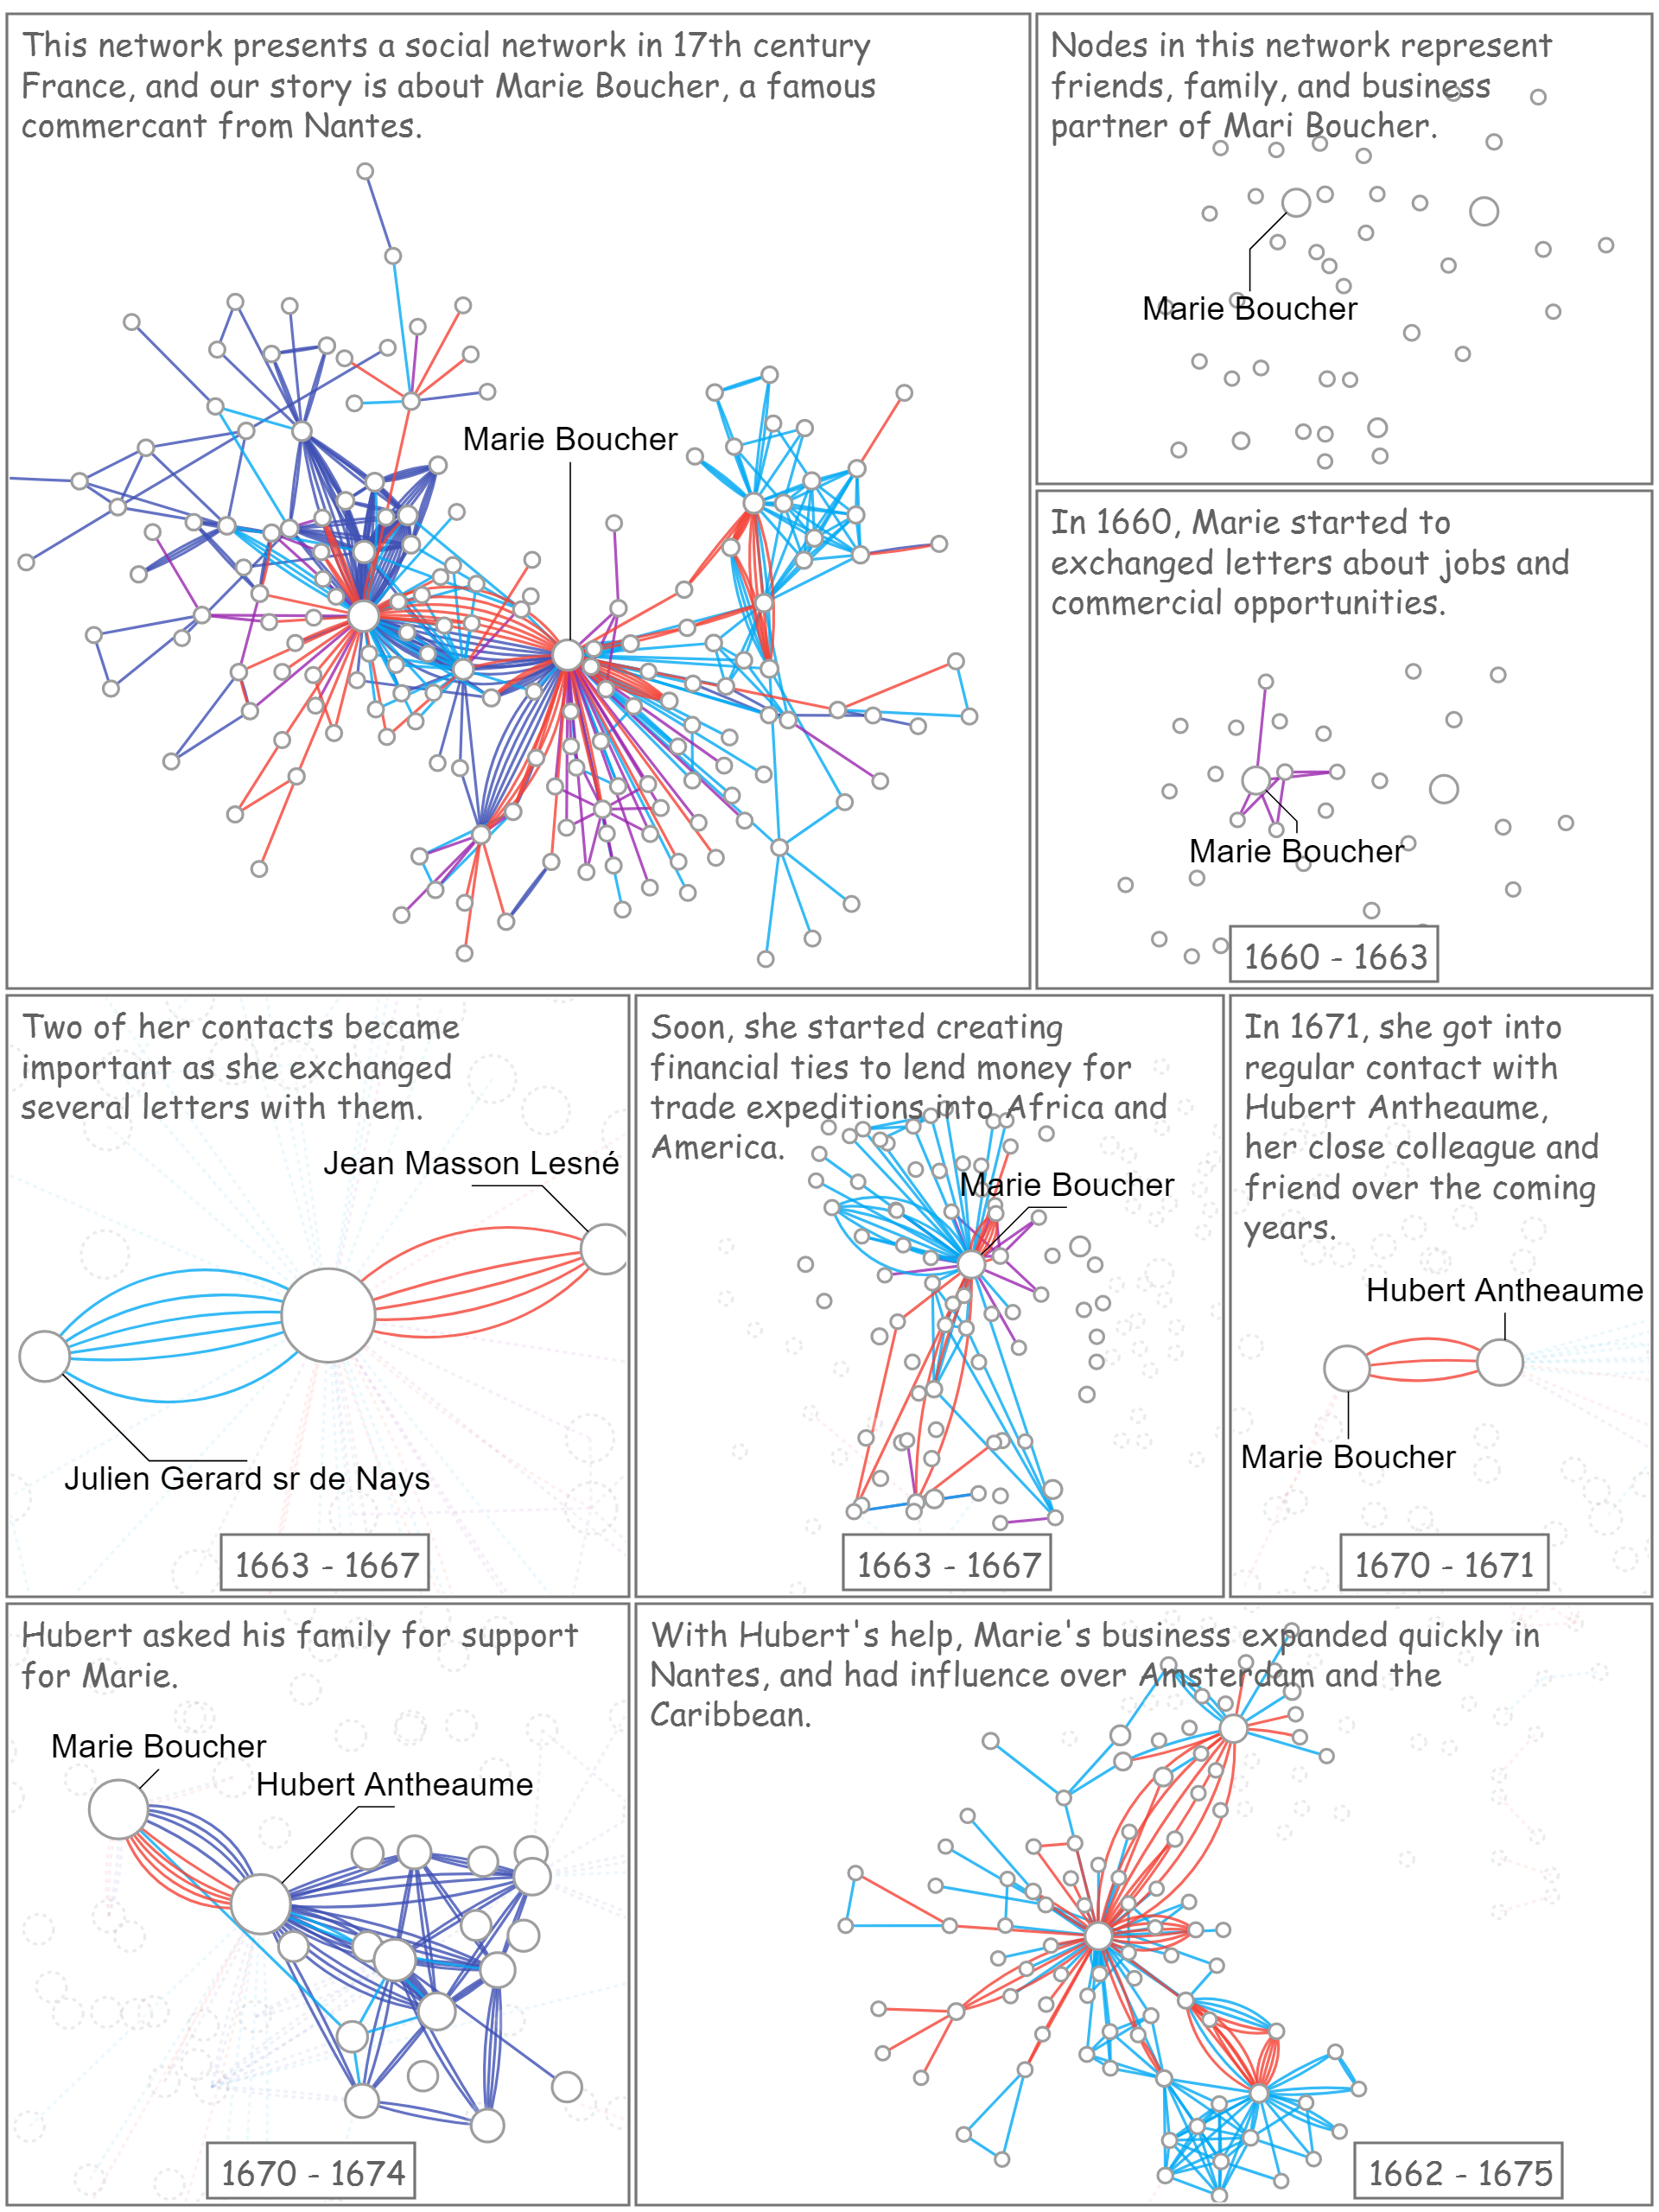
\includegraphics[width=0.25\textwidth]{figures/marie-boucher}
%     }
% \vspace{-0.1cm}
%     \caption{Six examples of data comics created with \toolname{} using different datasets. Higher resolution versions are available in supplementary material as well as on \url{https://datatoon.datacomics.net}. }
%     \label{fig:examples}
% \end{figure*}

% \begin{figure}
%  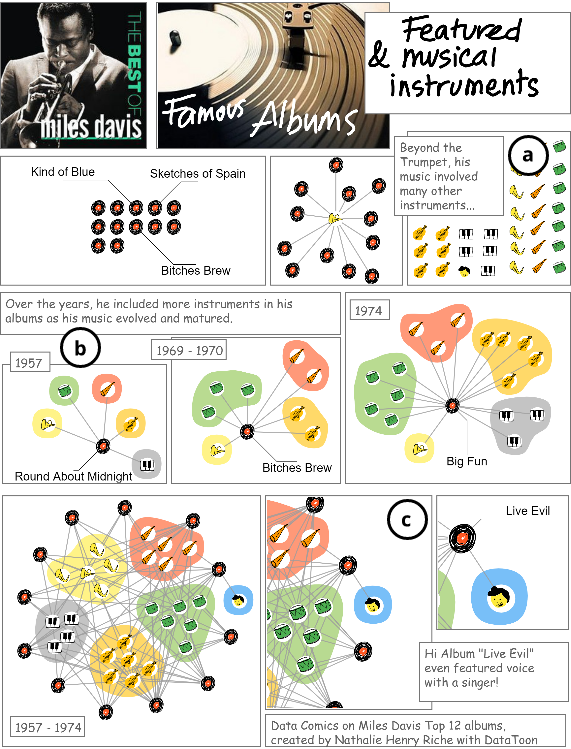
\includegraphics[width=\columnwidth]{figures/milesdavis-2.png}
%   \caption{Data Comics created with DataToon featuring (a) expressive visuals for representing instruments (C1), (b) breakdown of pane to convey temporal evolution (C2), (c) transition between panels at different scales (C3), laid out in 2D space to convey a linear story (C4).}
%   \label{fig:miles}
% \end{figure}

% \section{Examples}

% To demonstrate the expressiveness of comics that can be created with DataToon, we assembled a gallery available in supplemental material.  Figure~\ref{fig:examples} presents six comics showing multivariate and temporal social networks and co-authorship networks, as well as networks depicting relationships around movies, actors, and directors. We refer to the specific comics in Figure~\ref{fig:examples} through letters (a-f) in this section.

% DataToon supports different styles ranging from sketchy (a,d), to clean vector-graphics (e,f), including pictures (c), as well as small pictograms for nodes (b,c,d,e). Free placement of panels allows for a variety of layouts such as described in ~\cite{bachdesign}; tiles implying a clear sequential narrative (e.g., a,b), larger panels for an overview and smaller for details (b,c). Comic (d) still employs a sequential layout but aligned in a clock-wise manner to break the convention of the zig-zag layouts. Some of the comics use sequence (panels) to show temporal evolution (d,e,f), others imply different facets (a) and details of the data (b,c). 



% \rev{or add user driven examples here?}

\section{Evaluation}

Our evaluation methodology is representative of other recent evaluations of visualization authoring systems~\cite{ren2018beliv}, in that we demonstrate the {\it expressiveness} of \toolname{} with an example gallery (\autoref{fig:examples}) and
% , where Ren~\etal~\cite{ren2018beliv} define expressiveness as the scope of possible visualization design choices enabled by a system. 
also evaluate its {\it learnability} and {\it usability} via a reproduction study.

\subsection{Example Gallery}
% \nam{do we need to say this: While we did not formally evaluate the range and expressivity of data comics created with \toolname{}, several co-authors, co-workers, and participants of the study used it to create comics; \autoref{fig:examples} showcases some of these.} 
\rev{\autoref{fig:examples} shows example comics varying in their comic style, including diverse rendering styles (abstract, sketchy, realistic), panel layouts (inset, overlapping, staggered)~\cite{bachdesign}, visualizations (unit charts or pictographs, maps, set visualizations, node-link diagram), and narrative structures (overview+detail, nonlinear-temporal, cut-out, build-up~\cite{bachdesign}). The gallery also exemplifies a diversity of datasets, including multivariate and temporal social networks and co-authorship networks.}

% \deleted{The examples encompass a diversity of datasets, including multivariate and temporal social networks and co-authorship networks, as well as a variety of comic styles, ranging from sketchy to precise.} The gallery also exemplifies different narrative patterns~\cite{bach2018napa} showing temporal evolution or iteration over different dimensions of the data. 
%We also included videos of the authoring processes for these examples in our supplemental material.
%~\rev{can we?} \matt{As videos?}.
 
\subsection{Reproduction Study}
%\matt{This paragraph addresses R4's comments, who focused way too much on the study}
To evaluate whether people can learn how to use \toolname{} to create comics from data, we conducted a qualitative reproduction study, in which participants are asked to reproduce them completed examples with \toolname{}. 
This type of study is particularly common in the evaluation of visualization authoring tools~\cite{ren2018beliv}, having been used to evaluate Lyra~\cite{satyanarayan2014lyra}, ChartAccent~\cite{ren2017chartaccent}, DataInk~\cite{xia2018dataink}, Data-Driven Guides~\cite{kim2017data}, Data Illustrator~\cite{liu2018data}, and Charticulator~\cite{ren2018chart}. 

\vspace{2mm}
\bpstart{Participants} 
We recruited eight participants from a large software company in the United States. Half of the participants were graphic designers with limited data literacy (P1-P4: 3M, 1F; ages 30$\--$50, avg: 44), while the other half were data analysts with minimal experience in design tools (P5-P8: 2M, 2F; ages 31$\--$42, avg: 37). 

\vspace{2mm}
\bpstart{Apparatus}
Participants used a earlier version of \toolname{} on a Microsoft Surface Studio with a 28-inch screen at 4500 $\times$ 3000px (192 PPI), a device that enables simultaneous pen and multi-touch input.

% From the graphic designers we sought to gather feedback on the interface paradigms we selected and implemented in \toolname{}, to assess if key interactions or concepts were missing to produce data comics, and to gain an understanding of how it compares with tools that are more oriented to graphic design. From the data analysis, we aimed to assess whether they can learn \toolname{} and use it to create comics from data without guidance.  

%\bstart{Participants}
% We recruited our eight participants from a large software company in the United States. The graphic designers (P1-P4: 3 males, 1 female, aged 30 to 50, average 44) had professional experience in graphic design (e.g. over 20 years of experience using Adobe Illustator). Three of them had relatively low expertise in data analysis but one reported creating charts from data on a monthly basis. The data analysts (P5-P8: 2 males, 2 females, aged 31 to 42, average 37) perform data analysis and create charts and visualizations as part of their job. They had low or no experience with graphic design tools. All participants received \$20 in lunch coupons for their time. Three of our participants were left-handed.

%\bstart{Apparatus}
% We used a Microsoft Surface Studio with a 28 inch screen at 4500$\times$3000px (192 PPI) enabling simultaneous pen and multi-touch input.

\vspace{2mm}
\bpstart{Procedure and tasks}
Beginning with a demographic survey, each study session lasted $\sim$90 minutes, with two participants finishing in $\sim$60 minutes, and one taking $\sim$120 minutes. \rev{We asked them to reproduce two comics: 1) the first with guidance from us using the comic about \textit{World War I alliances} (\autoref{fig:interface}) and 2) the second without any assistance using the comic inspired by Fathom's {\it Scaled in Miles} project~\cite{fathom} about the evolving instrumentation on Miles Davis' records (\autoref{fig:examples}-left).
The first task served as a training session and lasted 30 to 40 minutes, which included a 15-minute tutorial, while the second task lasted between 30 and 50 minutes.} The study ended with three Likert-style questions about ease of use \& learning, and enjoyment, along with a semi-structured interview about their experience.
%using \toolname{}.

% In the beginning, the experimenter asked each participant to complete a demographics questionnaire, then asked them to create two data comics (\#1,\#2) with \toolname{} and concluded with three 7-point Likert scale questions (ease of learning, ease of use and enjoyment) as well as a short interview. %\ben{on the tool, I guess?}
% \bpstart{Comic \#1: Demonstration and exploration} 
% In this first task, we asked participants to reproduce the data comic from our usage scenario about \textit{World War I alliances} (\autoref{fig:interface}), which we provided as a printout. We encouraged participants to experiment with \toolname{} until they felt comfortable to proceed without additional guidance from us. This task served as a training session and lasted 30 to 40 minutes, which included a 15-minute tutorial.
% about the capabilities of \toolname{}.


% With the first comic, participants had to replicate a data comic on \textit{World War I alliances} depicted in \autoref{fig:tool_overview} and provided as a print out.  This phase served as a tutorial and training for participants to learn and explore what was possible with \toolname{}. The experimenter presented the main principles of the interface and demonstrated the interactions required to create comics. At the end of this tutorial, participants started from a blank page and proceeded to recreate the comic, asking questions as needed. Participants were encouraged to try their own experiments with the tool until they felt comfortable to proceed without guidance. This first task lasted 30 to 40 min (including the 15 min tutorial).

% \bstart{Comic \#2: Replication without guidance}
% In the second task, without any guidance from us, we asked participants to reproduce a data comic inspired by Fathom's {\it Scaled in Miles} project~\cite{fathom} about the evolving instrumentation on Miles Davis' records (\autoref{fig:examples}-left); as with the first task, we provided the completed comic as a printout. We asked participants to think aloud as they worked, and we proceeded to observe and note usability issues, participants' utterances, commonly used features, as well as features that were left unused. This task lasted between 30 and 50 minutes.

% This time, the experimenter did not offer any guidance. 

\subsection{Observations}
All participants successfully completed both comics, while we discovered several usability insights into the usability of \toolname{}. We describe our observations below.

% P2 required a few hints to recall how to achieve some design elements in the second task.
% Based on the Likert responses, participants found \toolname{} to be easy to learn and use and they enjoyed using it.
% at 5.6/7 for ease of learning, 5.9/7 for ease of use, and 6.5/7 for enjoyment.

% Seven participants used \toolname{} without any guidance from the experimenter to replicate the second comic. 

% One participant required a few hints to recall how to complete certain interactions. On average, participants rated \toolname{} at 5.6 out of 7 for ease of learning and 5.9 out of 7 for ease of use. %\ben{What about 'enjoyment'?} We now discuss additional findings. 


%problem with conflicting interaction paradigm of the OS - pen as stylus
%P7 wanted to use pen as a stylus (right after draggging from folder)

\vspace{2mm}
\bpstart{Learning to interact with both pen and touch}
All of the participants appeared to grasp \toolname{}'s interaction design by the end of the study, except for P2, who had no prior experience with pen + touch devices. It took a long time (approx. 10 min) for P2 to complete the first task and the effort spent to learn the interactions are reflected in their low ease of learning (3/7) and use (4/7) scores. P4, P5, P6, and P7 also repeatedly appeared to be frustrated when attempting to use pen and finger interchangeably, with P7 stating \textit{``I kept using my hand instead of the pen''}.

% Other participants made minor comments 

Participants bimanual pen and touch interaction to be engaging, with P8 remarking on the simplicity of the interactions: \textit{``I love the power of just dragging} [shows fingers] \textit{and creating} [shows the pen]\textit{''}. P4 spoke about the empowering experience of bimanual pen and touch input for content creation, making \toolname{} \textit{``unique''} and \textit{``fun''} compared to other tools: \textit{``I feel like a surgeon because I got precise and used both of my hands, not something I do ever. It's pretty cool!''}.
% While not complained, we also observed several other participants (P4, P5, P6, P7) repeatedly had issues by trying to use pen and finger interchangeably. 

% During the first task, We also observed that several other participants  repeatedly having issues with bimanual interaction.

% Their additional learning effort was reflected in the time to complete the first task (10 minutes longer than other participants) and the final ratings, 2 to 3 points lower than other participants for ease of learning (3/7) and ease of use (4/7). 

% During the first task, the experimenter also observed four other participants (P4, P5, P6, P7) repeatedly having issues mastering bi-manual interaction. The main issue faced by all participants was the desire to use pen and finger interchangeably.  However, only P2 and P6 reported it as a significant usability issue in the interview: \textit{``I kept using my hand instead of the pen''}.

% From the other six participants, we received many comments on the benefits and the engaging nature of bi-manual pen and touch interaction, once mastered. This is also reflected in the final ratings as the average enjoyment of using our tool is over 6 out of 7. 

% P8 commented on the simplicity of the interactions: \textit{``I love the power of just dragging} [shows fingers] \textit{and creating} [shows the pen]\textit{''}. P4 commented on the empowering experience it provided, making the app \textit{``unique''} and \textit{``fun''} compared to other tools: \textit{``I feel like a surgeon because I got precise and used both of my hands, not something I do ever. It's pretty cool!''}.

\vspace{2mm}
\bpstart{A focused tool set for design exploration}
The graphic design participants all expressed that one notable strength of \toolname{} was a \textit{``focused tool set''} (P1), its interface \textit{``streamlining the set of tools''} (P4) compared to existing illustration tools. We observed that our interface enabled alternative workflows to achieve the same result, reflecting what Ren~\etal~ refer to as the {\it flexibility} of a visualization authoring tool~\cite{ren2018beliv}. For example, several participants began with multiple panels, adjusted the content of each panel before customizing each of them in turn. Others would create and modify one panel until it was polished, only then duplicating to instantiate the next panel.

% Three of our graphic designers also commented that the look and feel of the interface, \textit{``the soul of the app, this handwritten feel''} (P1), and sketching on a canvas were features that encouraged them to explore, ideate, and generally experiment with different data comic designs.

% For example, all but one participant replicated the first comic using a different order of interactions than demonstrated by the experimenter. We also observed a large variation in working styles between participants. Design explorations also varied from participants: some created many panels, altering and erasing them and recreating new ones to iterate while other participants worked mostly in a single panel, extensively using the undo/redo feature. 

% One particular challenge for those using these types of authoring interfaces (having a focused set of instruments with different functions, as opposed to an exhaustive set of menus and buttons) is that it may prove intimidating upon first use, since many functions are hidden. This was particularly true for our data analysts. \textit{``Minimalism is in, it looks just like a simple drawing app, but then it can be intimidating because how do you achieve all of this?} [pointing to print out of the data comics] \textit{I was nervous''} (P8). However, it is worth noting that all participants mastered the interface after the first task.

Participants' difficulties often related to feature discoverability, as not every pen mode was visually shown in the interface. For example, in the version of \toolname{} used in the study, the pen button was used to activate the highlight pen. P8 commented that \textit{``Minimalism is in, it looks just like a simple drawing app, but then it can be intimidating because how do you achieve all of this?} [pointing to print out of the data comics] \textit{I was nervous''}. Similarly, P1 commented that the principle of dragging and dropping elements into panels was violated in the case of time captions, which required a double tap, making it challenging to discover. 



% small inconsistencies in interaction principles can rapidly degrade the experience and make it hard for participants to remember how to perform specific operations.

% For example, P3 noted that an inconsistency where holding the pen button selected items when in pencil mode but it inked when used as a highlighter, which caused him to repeatedly make errors in the tutorial. P1 also commented that the general principle of dragging and dropping elements into panels was violated in the case of time captions, which required a double tap, which made it particularly challenging to remember. 



%P5  also expressed doubts on remembering \textit{"the huge number of interactions"} but commented that he remembered more than he originally thought.


%Another challenge, for our data analysts (P5-P8), who were unfamiliar with graphic design and sketching apps, is that 
%on remembering the \textit{"right order of instructions"}, taking a deep breath and stating ~\textit{"Now that's the hard part [make the largest illustration of Miles Davis albums]"} but then he proceeded to complete the panel in less than ten minutes and expressed surprised and proudness of his illustration. 

%- P1 and P4 noted the "focused toolset" (P1) streamlining the set of tools to learn and use for a specific task. 
%- P1 on time label generation (double tap inconsistent from other gesture) "if your remember that, that is really cool"
%- graphic designer P3 pointed out inconsistency in holding button to ink instead of select in annotation mode

%-P8 "When I looked at this [print out of comics], I thought it would be difficult but it is not as I thought it would be"
%- minimalism (just different instruments) but for non experts it could be intimidating


%- p3: like the richness in expressiveness, more freedom than with other tools, sketchy prototyping feel. lots of potential in this vein. 
%- P1 on captions "I feel like this one I want to handwrite it" -> turn font into sketchy. P1 "This is kind of the soul of the app: getting this handwritten feel"
%- P6 "Now, I'm going creative" "When I said I was no artist, that's it" "Oh it does not look that bad"



\vspace{2mm}
\bpstart{Closing the gap between analysis and storytelling}
Participants appreciated the ability to discover patterns during the story authoring process, suggestive of a possible advantage over visualization authoring tools that are disjoint from data analysis tools. We observed that data analysts tended to explore the data before constructing on their comics. For example, P5 started by creating many panels (one per node type) and by commenting on the structural patterns in the data. P8 used a different strategy, adding each node type to a single panel in succession, where each node type was a different instruments featured on Miles Davis records; upon doing so, P8 stated that \textit{``now I am beginning to see the relationships between instruments [...] I am going to move things around so I can understand my data''}. Finally, some participants noted the necessity of additional data abstraction. For example, P3, looking at a particularly dense node-link diagram, said \textit{``I wish there were a way to untangle that because that is a super full graph''}, suggestive of a need for capabilities that aggregate nodes and links.
\vspace{-0.2cm}


%- P8 "I am scared to erase" (thought she would loose her data)

% Data analysts (P5-P8) particularly enjoyed using \toolname{} (rated enjoyment as 6.5/7 on average), many commenting that they were not artists or did not know how to draw but yet made aesthetically pleasing visuals: \textit{``the appearance of the cartoons was much nicer than I could have created''} (P7). P8 also noted that she liked \textit{``being shielded from all the data complexity and just focus on presentation''}.
%- p7 "When can I have it"

%- for data analysts feels like they can focus on presentation (shield them from data complexity)
% As participants created comics, we gathered a number of comments on the possibility to transform visual representations of data into more ``designed'' illustrations to make insights more salient. 

% For example, P3, looking at a particularly densely connected node-link diagram, commented \textit{``I wish there was a way to untangle that because that is a super full graph''} and asked if we had features (such as bundling or link aggregation) to simplify the visualization in places to illustrate that two of its clusters were highly connected. P3 then reflected that \textit{``there is an interesting balance between what I want to provide you with a sketch to give you a general idea of the data but not show ALL the data''}.  We believe that supporting this subtle shift from data visualization towards what we call \textit{information design} is an interesting direction for future work.
\vspace{2mm}

\subsection{Lessons Learned from the Reproduction Study}

\rev{The results of the study illuminated a set of usability insights regarding the difficulty of discovering features, the inconsistency of pen and touch interactions, and the complexity of visualization contents. These insights led to several improvements to the design of \toolname{}.}

\rev{To address the feature discoverability issue, we ensured that all pen modes are visible (\autoref{fig:interface}A) without cluttering the interface and degrading the authoring experience. In addition, after observing participants repeatably attempting to use fingers where we enforced use of the pen, which initially included panning and zooming panel content, we opted to accommodate more touch interaction, reflecting \textit{the pen writes, touch manipulates} mantra~\cite{hinckley2010pen}. We also replaced the double-tap gesture for creating time captions with a consistent drag gesture. Finally, to handle the visual complexity issue, we added the ability to filter nodes of interest from a panel, as well as the panel suggestion functionality for assisting with exploring complex data.}






% Based on the observations and feedback from the reproduction study, we made several improvements to \toolname{}. The previous version of \toolname{} used in the reproduction study is available as supplemental material for comparison. %\matt{release process for a website will not be done in time for a CHI submission} 
% First, after observing participants repeatably attempting to use fingers where we enforced use of the pen, which initially included panning and zooming panel content, we opted to accommodate more touch interaction, reflecting \textit{the pen writes, touch manipulates} mantra~\cite{hinckley2010pen}. To address the feature discoverability issue, we ensured that all pen modes are now visible (\autoref{fig:interface}A), without cluttering the interface and degrading the authoring experience. We also replaced the double-tap gesture for creating time captions with a consistent drag gesture. We also added the ability to filter nodes of interest from a panel. Finally, we added the panel suggestion functionality for facilitating rapid and iterative storyboarding (C4). 

% \rev{add deployment in the wild and user driven examples}



% - phase 1 participants used tools in different orders than demonstrated.
% - participants with no data expertise required more explanation about data.  
% - from graphic design participants, we solved a few bugs and added the following features to the tool: lock, undo, sketchy font
% - three left-handed participants  (PXXX) suffered a bit from the zoom slider
% - participant who had no previous pen and touch experience (P2, others?) struggled with bimanual interaction
% - participants all co-adapted to zoom interaction although X of them started repeatedly using pinch and zoom in panel

% graphics:

% Easy to learn: 1 (p1), 5 (p2), 3 (p3), 2 (p4),       2 (p5), 1 (p6), 2 (p7), 3 (p8)
% Easy to use: 2 (p1), 4 (P2), 2 (p3), 1 (p4),         2 (p5), 3 (p6), 1 (p7), 2 (p8)
% Enjoyment: 1 (p1), 3 (P2), 3 (p3), 2 (p4),           2 (p5), 1 (p6), 2 (p7), 1 (p8)

% - P1 struggled with aligning panels exactly and was frustrated when it moved -> lock- P1 and P3 noted that the concept of selections (selecting multiple objects) and layers was missing from the tool compare to more advanced one. P1 "I feel there could be a selection paradigm to apply operations to a group [of nodes]"
% - other did express frustration with not snapping aligning in grid (PXXX?)
% - P1 loved duplicating panels "I"
% - P1 on label creation "very fluid. You get something for nothing with that gesture" 
% - P1 "This is a really satisfying visual. I like the color palette and the shapes of what I made here".
% - P2 had no experience with pen and touch and found it difficult to remember that the touch and pen were doing different actions. see lowest rating in easy to learn and use.
% - P2 had also no experience with data analysis and chart creation, 
% - P2 and P3 frustrated that you had to set the color a priori and could not edit (had to remove group, change color and recreate group)
% - P2 wanted more functions to change fonts etc
% - confused with the data binding P2 "I thought the legend is something you made" "you don't really know how the data is impacting things"
% - p3 why need to use the pen tool to pan and zoom? why not use fingers
% - p3 "I wish I could group panels a posteriori"
% - p3 "I am not sure how do i know which mode I am in"
% - P3 on easy to learn: small toolset but "even after the tutorial I made mistakes"
% - p3 on enjoyment "with pressure it might be frustrating" (like aligning panels etc). 
% - p3 reminded him as adobe creative studio beta - same level of polish. lots of potential but missing sophisticated features like font management, symbols, guides, layers, assistive drawing.



% \section{Examples}
% \ben{Shouldn't this section go before the study eval? }
% \nam{let's remove this section and refer to the example figure somewhere else (probably in the discussion}

